\documentclass[9pt]{report}

\usepackage{talks}
\newcommand{\expect}[1]{\mathbb{E}\!\left[ #1 \right]}
\newcommand{\reals}{\mathbb{R}}
\newcommand{\draw}[2]{#1^{(#2)}}
\usepackage{mathpazo}
\usepackage{sourcecodepro}
\usepackage{tikz}
    \usetikzlibrary{positioning, shapes, arrows.meta}

\begin{document}

\sf \mbox{}
\\[12pt]
\spc{{\LARGE\bfseries \color{MidnightBlue}{Language models for statisticians:}}
\\[4pt]
\spc{\Large\bfseries \color{MidnightBlue}{from $n$-grams to
    transformers to chatbots}}
\\[24pt]
\noindent 
\spc{\large\bfseries \color{MidnightBlue}{Bob Carpenter}}
\\[2pt]
\spc{\small Center for Computational Mathematics}
\\[-1pt]
\spc{\small Flatiron Institute}
\vfill 
\noindent 
\spc{\footnotesize July 2023}
\hfill

\includegraphics[width=1.25in]{img/flatiron_logo.png}

\sld{What is a language model?}
\begin{itemize}
\item \myemph{Language} uses a \myemph{finite} number of
  symbols called \myemph{tokens}
  \subit{we assume a finite \myemph{token set} $\mathsf{Tok}$ of size $K$}
\item Tokens may be letters, words,
  sounds, syllables, etc.
  \begin{subitemize}
  \item letters or words traditional (e.g., Shannon 1948)
  \item GPT uses \myemph{sequences of letters} (average 1.5 tokens per
    English word)
  \end{subitemize}
\item Treat language as a \myemph{stochastic process}
  \subit{$Y = Y_1, Y_2, \ldots$ for random variables $Y_n \in T$}
\item Models typically \myemph{autoregressive}, predicting next
  word from previous
\end{itemize}

\sld{$K$-gram language models \hfill \normalsize{(Shannon 1948)}}
\begin{itemize}
\item Assume language process is \myemph{order-$K$ Markov}
  \begin{subitemize}
  \item tokens conditionally independent given previous $K$ tokens
    $$
    p(y_n \mid y_{n-1}, \ldots, y_1)
    = p(y_n \mid y_{n - 1}, \ldots, y_{n - K}).
    $$
  \end{subitemize}
\item Even \myemph{GPT is Markovian}
  \begin{subitemize}
    \item Chatbots use $N = 4096$ (GPT-3) or $N = 8192$ (GPT-4)
    \item API provides $N = 32,768$ GPT-4 and $N = 8192$ code specialization GPT-3
    \item cf. a real computer is technically a finite-state machine
    \end{subitemize}
  \item Limited context allows relatively \myemph{efficient algorithms}
\end{itemize}
    
\sld{Shannon's $K$-gram models}
\begin{itemize}
\item \myemph{Claude Shannon}. 1948. \myemph{A Mathematical Theory of Communication.}
  \textit{Bell System Technical Journal}.
\item Shannon considered English \myemph{letters} ($K = 1, 2, 3$) and
  words ($K = 1, 2$)
\item \myemph{What is English?}  How do we collect a \myemph{sample}?
\item Shannon used \myemph{books of frequencies}
  \begin{subitemize}
  \item \myemph{letter trigrams} (1939 book); \myemph{word bigrams} (1923 book)
  \end{subitemize}
\item Fit and inference usually \myemph{regularized MLE}
  \begin{subitemize}
  \item ensures \myemph{non-zero probability} for any sequence
  \item (non-parametric) \myemph{Bayes} usually too \myemph{expensive}
  \item often \myemph{heuristic driven} for efficiency (e.g., speech to text)
  \end{subitemize}
  
\end{itemize}

\sld{Shannon's fit}
\begin{itemize}
\item MLE probabilities from compiled tables of letters (1923), words 
      (1939) 
    \subit{or, open books at random, find current context, generate 
        following word}
\item Shannon generated random examples
  \begin{subitemize}
    \item \myemph{Order 1, letters}: OCRO HLI RGWR NMIELWIS EU LL NBNESEBYA TH EEI ALHENHTTPA OOBTTVA
      NAH BRL.
    \item \myemph{Order 3, letters}: IN NO IST LAT WHEY CRATICT FROURE
      BIRS GROCID PONDENOME OF DEMONSTURES OF THE REPTAGIN IS
      REGOACTIONA OF
      % CRE.
    \item \myemph{Order 1, words}: REPRESENTING AND SPEEDILY IS AN
      GOOD APT OR COME CAN DIFFERENT NATURAL HERE HE THE A IN CAME THE
      TO OF TO EXPERT
      % GRAY COME TO FURNISHES THE LINE MESSAGE HAD BE THESE.
      \item \myemph{Order 2, words}: THE HEAD AND IN FRONTAL ATTACK ON
        AN ENGLISH WRITER THAT THE CHARACTER OF THIS POINT IS
        THEREFORE ANOTHER
        % METHOD FOR THE LETTERS THAT THE TIME OF WHO EVER TOLD THE PROBLEM FOR AN UNEXPECTED.
  \end{subitemize}
\end{itemize}

\sld{Measuring accuracy with entropy}
\begin{itemize}
\item Accuracy of $K$-gram language model $p_Y$ measured with
  \myemph{entropy (rate)}
\item Given a random sequence $Y \in \textsf{Tok}^N,$ its
  \myemph{entropy} in \myemph{bits} (base 2) is
  $$
  \textrm{H}[Y]
  \ = \ \mathbb{E}\!\left[ \log_2 p_Y(Y) \right]
  \ = \ \sum_{y \in \textsf{Tok}^N} p_Y(y) \cdot \log_2 p_Y(y).
  $$
\item The \myemph{entropy rate} is average entropy per token, $\lim_{N \rightarrow \infty} \,
  \textrm{H}[Y] / N,$
\item The entropy rate for $K$-grams is given by \myemph{conditional entropy},
  \begin{align*}
    \textrm{H}[Y_n \mid Y_{n - 1}, \ldots, Y_{n -K}]
    \ &= \ \mathbb{E}\!\left[\, \log_2 p(Y_n \mid Y_{n - 1}, \ldots,
        Y_{n -K}) \, \right]
    \\[4pt]
    &= \ \sum_{y \in \textsf{Tok}^{K + 1}}
    \ p(y) \cdot \log_2 p(y_{K + 1} \mid y_{K}, \ldots, y_1).
  \end{align*}
\end{itemize}

\sld{Entropy and compression}
\begin{itemize}
\item Shannon (1948) introduced \myemph{information theory} to model
  signal compression and decompression for communication
\item Assume a language model with pmf $p_Y$
\item Given a string $y \in \textsf{Tok}^*,$ the language model can be
  used to \myemph{compress} $y$ to $\lceil \log_2 p_Y(y) \rceil$ bits
\item Can be done in practice using \myemph{arithmetic
    coding} (Rissanen 1976; Witten, Neal, Cleary 1987) using
  \myemph{GPT output}
\end{itemize}

\sld{OpenAI's GPT-3: Published}
\begin{itemize}
\item \myemph{Training set} sizes \\[8pt]
  \small
  \begin{tabular}[t]{r|r}
    \myemph{Source} & \myemph{Tokens} \\ \hline
    Common Crawl & 410 billion  \\
    Books2 & 55 billion \\
    WebText2 & 19 billion \\
    Books1 & 12 billion \\
    Wikipedia & 3 billion \\ \hline \hline
    & $\approx$ 500 billion
  \end{tabular}
\item \myemph{Number of parameters}: $\approx$175 billion
  \vfill
\item \myemph{Context history size}: 4K tokens
\item Let's turn to \myemph{how it works $\ldots$}
\end{itemize}


\sld{Top-level architecture}
\hfill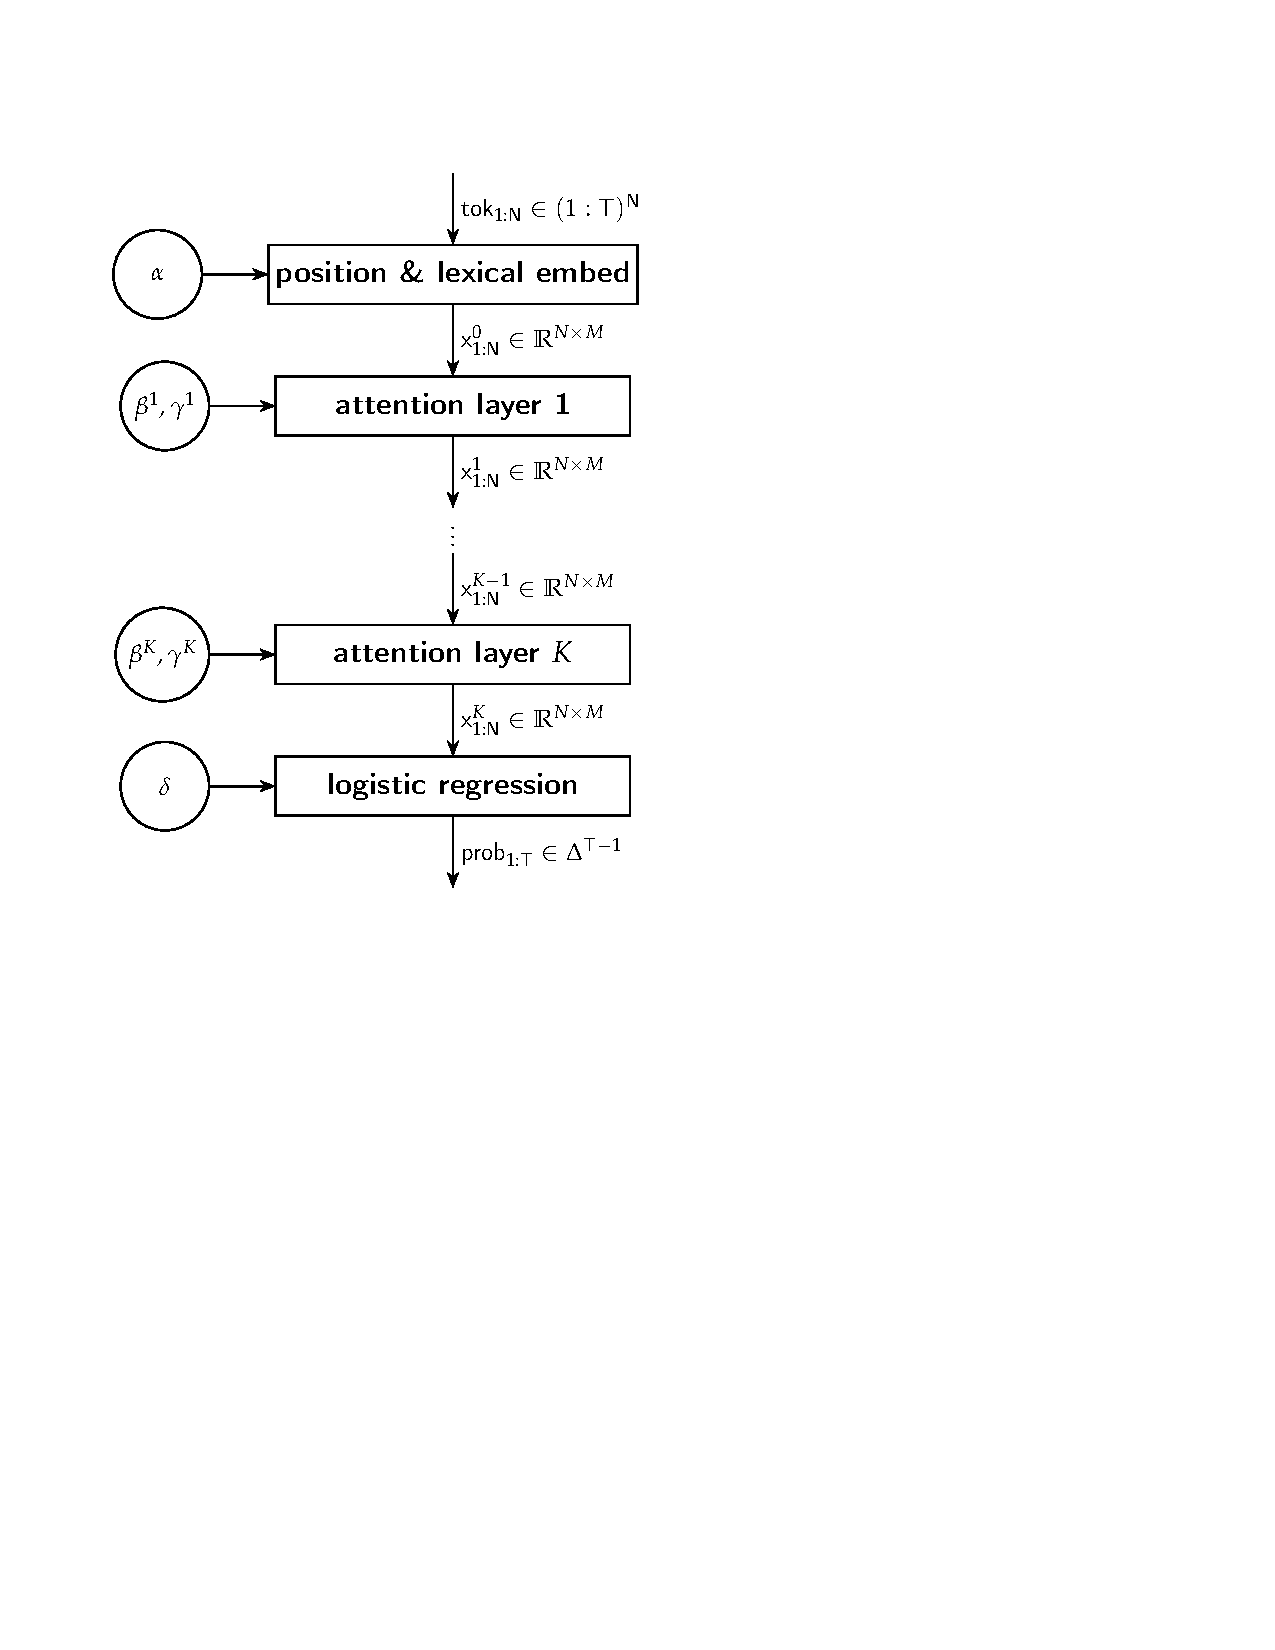
\includegraphics[height=\textheight]{img/transformer-diagram.pdf}

\sld{Attention architecture}
\begin{center}
\vspace*{-24pt}
\hfill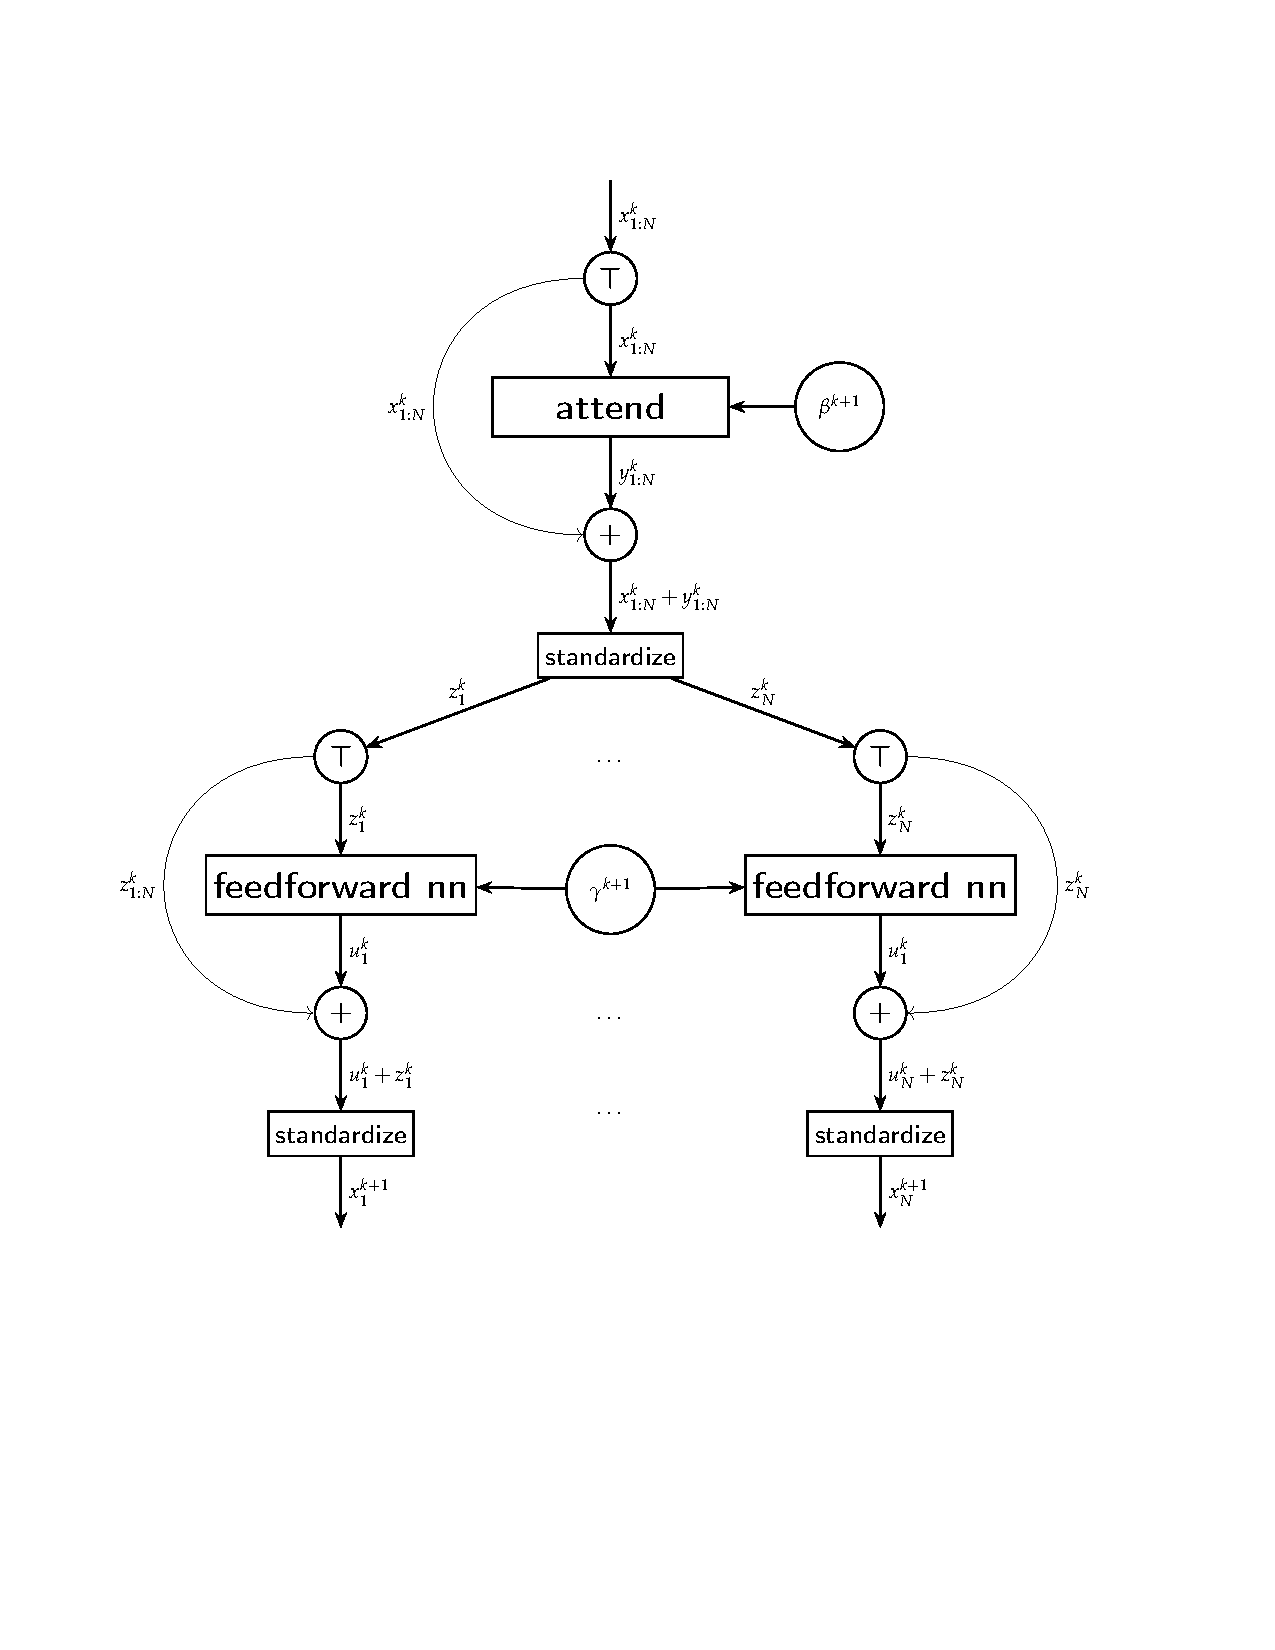
\includegraphics[height=\textheight]{img/attention-diagram.pdf}
\end{center}

\sld{Top-level pseudocode}
\footnotesize
\begin{center}
\begin{verbatim}
   DECODE(tok:  int<low=1,up=T>[N],    alpha:  matrix(T, V),
     betas: { query:matrix(K, V),  key:matrix(K, V),  value: matrix(V, V) }[A]
     gammas:  nn(V, L)[A],
     delta:   { 1: vector[T], 2: matrix(T, N * V) }):  simplex[T]
   -------------------------------------------
   for n in 1:N:                                         // for tokens:
       xs[0, n] = LEX(tok[n], alpha) + POS(n)               // embed
   for a in 1:A:                                         // for each layer:
       xs[a] = ATTEND(xs[a - 1], betas[a], gammas[a])       // attend
       for n in 1:N:                                        // for tokens:
           xs[a, n] = FEED_FORWARD(xs[a, n], gammas[a])         // shared nn
   y = STANDARDIZE(delta.1 + delta.2 * xs[A].flatten())  // GLM: linear layer
   return SOFTMAX(y)                                     // inverse link
\end{verbatim}
\end{center}
\normalsize

\sld{Lexical and positional embedding}
\footnotesize
\begin{center}
\begin{verbatim}
    LEX(t:      int<low=1,up=T>,
        alpha:  vector(V)[T]):  vector(V)  
    -----------------------------------------------------
    return alpha[t]                // one-hot

    POS(n:  int<low=1,up=N>):  vector(V)
    -----------------------------------------------------
    for i in 1:V / 2:
        r = n / N**(2 * i / V)      // pos / max_pos^(0..2]
        u[2 * i] = sin(r)
        u[2 * i + 1] = cos(r)
    return u
\end{verbatim}
\end{center}

\sld{Attention}
\footnotesize
\begin{center}
\begin{verbatim}
  ATTEND(x:      vector(V)[N],
         beta:   {query: matrix(K, V), key: matrix(K, V), value: matrix(V, V)},
         gamma:  nn(V, L)):  vector(V)[N]
  -----------------------------------------------------------
  for n in 1:N:                                         // for tokens:
      q[n] = beta.query * x[n]                              // embed query
      k[n] = beta.key * x[n]                                // embed key
      v[n] = beta.value * x[n]                              // embed value
  for n in 1:N:                                        // for tokenss:
      lp[1:n-1] = [q[n]' * k[1], ..., q[n]' * k[n-1]]      // attend log probs
                  / sqrt(V)                                //     scaled
      lp[n:N] = -inf                                         // mask future
      p = SOFTMAX(lp)                                        // attend probs
      u[n] = SUM(n in 1:N) p[n] * v[n]                       // weight vals
      y[n] = STANDARDIZE(u[n] + x[n])                        // residual + std
  return y
\end{verbatim}
\end{center}

\sld{Feedforward neural network}
\footnotesize
\vspace*{-6pt}
\begin{verbatim}
   FEED_FORWARD(x:     real[R], 
         alpha: { 1: real[S], 2: real[S, R], 
                  3: real[R], 4: real[R, S]):  real[R]
   ----------------------------------------------------
   u = alpha.1 + alpha.2 * x          // linear
   v = GELU(u)                        // nonlinear activation
   y = alpha.3 + alpha.4 * v          // linear
   return STANDARDIZE(x + y)          // residual + standardize

   GELU(v:  real[R]):  real[R]
       return [vi * Phi(vi) for vi in v]          // Phi(x) std normal cdf

   STANDARDIZE(v:  real[R]):  real[R]
       return (v - mean(v)) / standard_deviation(v)  // arithmetic stability

   SOFTMAX(real[R] v):  simplex(R)              // multi-logit inverse link
       return exp(v) / sum(exp(v))
\end{verbatim}

\sld{From LLM to Chatbot}
\begin{itemize}
\item \myemph{LLM goal}: predict \myemph{next token on web} page
\item \myemph{Chatbot goal} is to train a model that is
  \begin{subitemize}
  \item \myemph{helpful}: help users solve task
  \item \myemph{honest}: shouldn't fabricate or mislead user
  \item \myemph{harmless}: shouldn't cause physical, psychological,
    social, or environmental harm
  \end{subitemize}
\item Strategy is to \myemph{align} an LLM to be a Chatbot with
  \myemph{fine tuning}
  \begin{subitemize}
  \item LLM acts as an \myemph{informative prior}
  \item In ML terms, LLM provides \myemph{inductive bias}
  \end{subitemize}
\end{itemize}

\sld{Reinforcement learning with human feedback \\ \null\hspace*{1em}(RLHF)}
\begin{enumerate}
\item Supervised fine tuning
  \begin{subitemize}
  \item human raters \myemph{provide desired output} for sampled prompts
  \item \myemph{fine-tune} LLM with \myemph{supervised learning}
  \end{subitemize}
\item Reward model training
  \begin{subitemize}
  \item human raters \myemph{rank multiple outputs} for sample prompts
  \item train a \myemph{reward model}
  \end{subitemize}
\item Reinforcement learning
  \begin{subitemize}
  \item \myemph{policy ranks outputs} for sample prompts
  \item fine-tune LLM with \myemph{proximal policy optimization} (PPO)
  \end{subitemize}
\end{enumerate}

\sld{Some caveats}
\begin{itemize}
\item 
{\LARGE ``\null}This procedure aligns the behavior of GPT-3 to the \myemph{stated preferences of a
specific group} of people (mostly our labelers and researchers),\\[4pt] rather
than to any broader notion of `human values'.{\LARGE \null''} \hfill {\small (OpenAI 2022)}
\subit{cf. \myemph{Cultural consensus theory} provides mixture model of
  ``values''}
\vfill
\item {\LARGE ``\null}During RLHF fine-turning, we observe \myemph{performance
    regressions} compared to GPT-3 on certain public NLP
  datasets.{\LARGE\null''}
  \hfill {\small (OpenAI~2022)}
  \begin{subitemize}
    \vspace*{-12pt}
  \item i.e., performance degrades relative to unaligned model
  \item partially mitigated by \myemph{hierarchical modeling}
    alternating reinforcement and supervision
  \end{subitemize}
\end{itemize}

\sld{OpenAI's GPT-4: Unpublished}
\begin{itemize}
\item \myemph{Training set} unpublished (estimated $\approx$5 trillion)
\item \myemph{Parameter set} unpublished (estimated $\approx$2
  trillion)
\item \myemph{Context history size}: 8K or 32K tokens
\item \myemph{Hardware cost} training: $\approx$US\$500 million
  (incl.\ 10K+ US\$15K GPUs)
\item \myemph{Marginal cost} training: $\approx$US\$10s of
  millions (hardware, power, staff)
  \vfill
\item \myemph{Open AI (2023) now CLOSED}: {\small ``Given both
the competitive landscape and the safety implications of large-scale models like GPT-4, this report
contains no further details about the architecture (including model size), hardware, training compute,
dataset construction, training method, or similar.''}
\end{itemize}

\sld{The cat's out of the bag}
\begin{itemize}
\item Transformer LLM architecture published by \myemph{Google} (2017)
\item Alignment to ChatBots published by \myemph{OpenAI} (2022)
\begin{subitemize}
\item Meta (aka Facebook): \myemph{LLaMA}
  \vspace*{3pt}
  \begin{subitemize}
    \item \myemph{Open source} for research (since leaked)
    \item Stanford CS: \myemph{Alpaca} fine-tuned
    \item Runs 2 tokens/second on iMac with 4-bit floating point
    \end{subitemize}
  \item Google: \myemph{Bard}
  \item Google and OpenAI: \myemph{Copilot} (code/programming API integration)
\item Anthropic: \myemph{Claude} (100K token context) (branded as \myemph{Poe} for writing) 
\item Many smaller, less widely used alternatives
\end{subitemize}
\end{itemize}


\sld{References}
\begin{itemize}
\item Vaswani et al. (Google). 2017. \hfill (82K~citations) 
  \\
  \myemph{Attention is all  you need}. \textit{NeurIPS}.
\item Brown et al. (OpenAI). 2020.  \hfill (12K~citations)  
  \\ \myemph{Language models are few-shot
    learners}. \textit{NeurIPS}.
\item Ouyang et al. (OpenAI). 2022.  \hfill (1.5K~citations)
  \\
  \myemph{Training language models to follow instructions}.
  \textit{NeurIPS}.
\item Phuong \& Hutter (DeepMind). 2022.  \hfill (0.02K~citations)
  \\ \myemph{Formal algorithms for
  transformers}. \textit{arXiv}.
\item Bubeck et al. (Microsoft). 2023.  \hfill (0.4K~citations)
  \\ \myemph{Sparks of artificial general intelligence}. \textit{arXiv}.
\end{itemize}

\end{document}
